\documentclass[aip,amsmath, reprint, author-year]{revtex4-1}
\usepackage{url}
\usepackage[utf8]{inputenc}
\usepackage{hyperref}
\usepackage{graphicx} % for graphics
%\usepackage{listings} % for code listtings
%\usepackage{color}

%\setcitestyle{round, author-year}

\setcounter{page}{1}

%\bibliographystyle{aipauth4-1.bst}

\begin{document}

\begin{abstract}
An approach to generate generalised process capability data in order to populate and add functionality to a process capability database.
A description of the concept of generalisation, uses and implementation.
\end{abstract}

\title{Improving process capabaility database usage for robust design engineering by generalising measurement data}
\author{Andreas Bruun Okholm, s082562\\
Mathias Rask Møller, s082536\\
Thomas J Howard\\
Martin Ebro\\
Maria Holmberg}
\affiliation{Technical University of Denmark}
 
\date{\today}
\maketitle

%Introduction

\section{Introduction}

All manufacturing processes produce parts with variation from the specified dimensions. Understanding process variance and creating designs which are insensitive to the variance decreases cost of manufactured goods and increase user satisfaction. 
This is the main goal of the robust design methodology.
Early research focused on characterising the variance and understanding its relation to quality loss \cite{taguchi1986introduction}. 
During the 1990s many major American companies followed a trend of robust design and created process capability databases (PCDB), however due to the lack of practical tools for accessing process capability variation data these were largely unused for mechanical design purposes\cite{tata1999process}. 
While further research in PCDBs followed, it still seems there are challenges to be solved before widespread adoption in industry is possible.

In this paper, a literature review will be conducted on PCDBs looking at both challenges and proposed solutions. 
We propose a modified indexing scheme for PCDBs and couple it with a new measure of process capability, which is easily understood and directly applicable for the mechanical design engineer. 
This is one step to make it faster and easier for the mechanical designer to efficiently use process capability data in new designs. 

\section{Literature review}
Manufactured parts are designed with an allowable geometric variation. The outer limits of the allowable variation are the tolerances. The tolerances make sure the product will assemble and function as intended during use. In the early stages of new product designs tolerances are typically not taking into account. Instead the near final design will pass through a manufacturing or quality department, which will find and set the needed tolerances for the design to work as intended. This leads to very tight tolerances, which are very difficult and expensive to maintain in production. 

Robust design methodology focuses on creating engineering designs, which are insensitive to geometric variation reducing the need for tight tolerances. While the tolerances can generally be widened maintaining the same output performance, the goal is to find an optimum, which balances the cost of increased tolerance requirements, design complexity and the quality loss associated with design parameters being off target \citep{arvidsson2008principles}.

To estimate the optimum level of tolerances, knowing the current process capability data (PCD) is essential. “PCD is defined as the expected and obtained standard deviations and mean shifts for a feature produced by a particular process and made of a particular material” 
 \citep{tata1999process}.

There has been a significant amount of research, which shows use of process capability data to set correct tolerances will reduce rework, cost, failure rate, assembly problems and improve product performance  \citep{tata1999process}.
This will create a shift in design methodology, from ‘Design of Tolerances’, to ‘Design to Process Capabilities’ (DtPC). 

\subsection{Generating Process Capability Data}
In the 1990s, several papers were published on methods to predict process variation using process models  \citep{thornton2000use}. 

However creating process models can be very complicated and impractical for many manufacturing processes. Another option for acquiring PCD is to measure the actual process performance and store it in a database. In a typical manufacturing process multiple parts are measured during a first article inspection (FAI) and subsequently during routine process checks. 

From the measurement reports the mean shift $|\mu - m|$ and standard deviation $\sigma$ of the measurement set is calculated. 
Where $\mu$ is the process mean and $m$ the target dimension. This data is stored in the database along with the nominal size from a technical drawing and an index, which makes it possible to find the given data based on a combination of the feature, the features geometry, process and material attributes. 

\cite{thornton2004variation} combines the feature and its geometry/dimension into one index e.g. a hole and its depth or a chamfer and its angle. 

However creating process models can be very complicated and unpractical for many manufacturing process. 
Another option for acquiring process capability data is to measure the actual process performance and store it in a database. \cite{perzyk1998selection} describes such a database for storing general mechanical process capability data for the use of selecting optimal manufacturing methods.

\cite{kern2003forecasting}  proposed index scheme differs slightly, feature types are more abstract such as a front face or inner diameter. The geometry attribute is more generalized and loosely based on geometric product specification (GPS) e.g. the position or concentricity. This allows the engineer to easily search for a geometry attribute such as concentricity across many different feature types.

In order to do more advanced analysis, more data is often included in the PCDB including stock (the material stock type before processing), lower specification limit (LSL), upper specification limit (USL), machine, operator number, batch size and part volume.

The issue with these indexing schemes is that they are not very obvious and it is even ambiguous how to index a measurement set. To solve this problem \cite{kern2003forecasting} developed an assistance tool to aid the designer to select the correct index attributes. It seems the indexing schemes have become too complicated and abstract to be used efficiently. The issue of selecting the correct attributes arises every time a new design has to be evaluated in order to find the correct PCD. There is a tendency in robust design methodology towards applying robust design methods in the very early stages of product development \cite{ebro2012foundation}. If tolerance considerations should be included at this early stage the speed and ease of use of the PCDB is very important. 

\begin{figure}
\includegraphics[width=0.45\textwidth]{bias_std.pdf}
\caption{\label{fig:bias_std} Graphical display of process capability data as proposed by\cite{thornton2000use}}
\end{figure}

\subsection{Displaying Process Capability Data}
One way to make PCD more efficient to use is through clever graphical displays, which provides quick overview of important characteristics. \cite{thornton2000use} describes the development of a graphical view to show PCD. A x-y plot of mean shifts and standard deviation is showed for the selected measurement sets, see figure \ref{fig:bias_std}. 

Confidence intervals of both mean shift and standard deviation is shown for each measurement set to visualise the statistical significance. Guides shows which measurement sets could maintain a tolerance of e.g. $\pm 0.1 mm$. The view is great for the process engineer, showing overall process capability and indicating areas where easy gains in process capability is possible by adjusting the mean shift. 

However for the designer the plot is tedious to interpret, he is concerned with the actual tolerances possible for the given design and not the mean shifts and standard deviations.

% New Section 
\section{Improving Process Capability Database}
We will now present a concept of data indexing, processing and presentation, which tries to make it faster and easier for the designer to efficiently use PCD in new designs. The general principle is to provide an interface where the data is presented more generalised than typically done in PCDB interfaces. The indexing scheme is simplified, and made more flexible by using a tagging system. 

Instead of presenting the designer with statistical information, the recommended tolerances based on actual process capability are shown directly. The tolerances are normalised in regard to the specified dimension making more use of each dataset, minimising the risk of process capability requests not returning any results. Combined with advances in information technology we hope this will help make PCDBs viable in the early phases of product development as a robust design tool. Such a tool could also be basis for a PCDB driven tolerance estimation plugin for CAD software.

To test the system we have setup our own test database and populated it with measurement data. The PCD were created for this project and involved the measurement of 75 different samples from 4 different parts using a variety of different measurement techniques. The example data are further explained in section \ref{sec:result}.

\subsection{Indexing}

PCDBs need to be indexed to efficiently retrieve PCD of relevance to the current design. We propose to use material, process and geometry as the primary attributes. The material and process is defined as in previous work, e.g. the material could be ABS plastic and the process injection moulding. 

The geometry is the tolerance type, which is specified on the technical drawing. This includes the GPS tolerance options (e.g. concentricity or position) or just simple tolerances (e.g. distance, diameter). The direct relationship between the information on the drawings and the index attributes makes the selection of the correct geometry unambiguous. Another benefit of using the standard tolerance options is that the designers are already familiar terminology. 

This is combined with a tagging system, where additional tags can be inputted. Measurement sets affected by additional properties such as high length to width ratios or special surface treatment could be optionally tagged. Tags are not stored in the same manner in the database table as primary index and regular attributes, but in a separate table, which allows none or multiple tags to point to the same measurement set. This difference becomes apparent in the user interface where tags help the user to easily input additional information about the measurement set. The tagging system allows indexing design attributes that are specific to a single production method or material. E.g. for injection moulding it is possible to index the following design attributes:

\begin{itemize}
\item Material type of the mould: aluminium, steel, hardened, etc.
\item Mould/Process iterations (T0, T1, T2...) could give valuable insights of which specification limits require mould rework or process adjustment.
\item Tagging dimensions measured across parting lines could potentially show a general increase in desired specification limits. 
\end{itemize}

A complete database record of a measurement set can be seen in table 1 showing all of the input data of the measurement set.

\begingroup
\squeezetable

\begin{table*}
\begin{ruledtabular}
\caption{\label{tab:sampleset} Measurement set - As stored in the PCDB}
\begin{tabular}{lllllllll}
\textbf{Material} 		& \textbf{Process} 		& \textbf{Geometry}  		& \textbf{Target}  	& \textbf{USL} 		& \textbf{Mean Shift} & \textbf{Std.}   ${\sigma}$  \\
Thermoplastic 			& Moulding			& Diameter 			& 3.00			& 3.01			& -0.0486			& 0.0032				  \\
 - ABS, PC blend		& - Injection Mould.			\\
\\
\textbf{General Tag (1)} 	& \textbf{General Tag (2)} & \textbf{General Tag (3)}  & \textbf{Meas. Equipment}  	& \textbf{LSL} & \textbf{Measurement Date} 	& \textbf{N samples} \\
Mould Type			& inside				& Production run		 & CT Scanning			& 2.99		& 13 oct. 2013  			& 12\\
- Steel 				& 					& - PR3				 & Zeiss metrotom 800\\
- - NAK80 
\end{tabular}%
\end{ruledtabular}
\end{table*}
\endgroup


\subsection{Processing Capability Data}

Processing the capability data consists of three steps, detailed in the following sub sections:

\begin{enumerate}
	\item Compute the process capability specification limit (PCSL). 
	\item Normalise the PCSLs so it is independent of dimension. 
	\item Fit operating curves to the PCSL data grouped by different design attributes. 
\end{enumerate}

\subsubsection{Process Capability Specification Limit}
The process capability indices ($C_p$ and $C_{pk}$) described by \cite{kane1986process} and further developed \citep{wu2009overview}  ], have been widely adopted in statistical process control. Instead of looking at process mean $\mu$, standard deviation $\sigma$ and specification upper and lower limits $USL$, $LSL$ using process capability indices (PCIs) transforms these values into unit less numbers, which provides a quick overview of how a process is performing.

For an example, the commonly used PCI:

\begin{equation}
	C_{pk} = \frac{d - | \mu - m|}{3 \sigma} \nonumber
\end{equation}

where $d = (USL−LSL)/2$ is half the specification limit and $m = (USL + LSL)/2$ is the midpoint between the specification limits. This can be reversed for a known $C_{pk}$ to calculate the desired symmetric tolerance.

\begin{equation}
	d = 3 C_{pk} \sigma + | \mu - m|
\end{equation}

To highlight the difference between $d$ used to calculate PCIs, and $d$ used as an estimator for symmetric tolerances based on PCD we have named the variable process capability specification limit ($PCSL$). Using the data from table \ref{tab:sampleset} and a $C_{pk} = 1,66$. The PCSL is computed:

\begin{align*}
PCSL &= 3 \cdot 1.66 \cdot 0.0032 \, \mathrm{mm}
+ |0.0486  \, \mathrm{mm}| \\
&= 0.0645  \, \mathrm{mm}
\end{align*}

The recommended tolerance for the measurement in table  \ref{tab:sampleset}  is $3 \ mm \pm 0,0645 \ mm$. 

There are several commonly used PCIs each serving their own purpose  \citep{wu2009overview, taguchi1986introduction};
\begin{itemize}
	\item $C_a$ : Closeness of process mean to target 
	\item $C_p$ : Process precision 
	\item $C_{pk}$ : Amount of nonconforming (\%NC)
	\item $C_{pm}$ : Value loss (Taguchi loss function)
	\item $C_{pmk}$: Version of $C_{pm}$,  sensitive to mean shift. 
\end{itemize}

The difference between the different CPIs can more clearly be understood by looking at figure \ref{fig:CPI}, where the relationship between closeness to target $C_a$ and the standard deviation \sigma normalized using the half specification width $d$ is shown. The line for $C_{pm}$ is below that of $C_{pk}$ except for values of $C_a$ close to 1. Using $C_{pm}$ will in general be more conservative resulting in larger specification limits than $C_{pk}$. $C_{pkm}$ combines the value loss function $C_pm$ with the relation to yield of $C_pk$. $C_pkm$ is very conservative. For higher CPI values this effect is more pronounced.


\begin{figure}
\includegraphics[width=0.45\textwidth]{cpm_cpk.pdf}
\caption{\label{fig:CPI} Comparison of the different process capability indices.  }
\end{figure}

For the purpose of our database we have chosen to use $C_{pk}$, since it provides the most understandable result directly related to the yield of the process. The yield of a process is within
\begin{equation}
	2\Phi(3C_{pk})-1 \leq \text{yield} < \Phi(3C_{pk}) \nonumber
\end{equation}

where $\Phi(x)$ is the cumulative distribution function of the standard normal distribution N(0,1) \citep{boyles1991taguchi}. 

The optimal process capability index value depends on the application, however there exists a quality control practice called six sigma ($6\sigma$).  This advocates a target of $C_{pk} = 2$ (equivalent to $6\sigma$) for short term process capability, which has been shown to generally improve manufacturing quality and profits \cite{koch2004design}.

It is assumed that the process drifts over time up to $1,5 \ \sigma$ (effectively resulting in a sigma level of $4,5$), which still results in an acceptable $3,4$ ppm defects. For the $PCSL$ to reflect six sigma production capability, the $C_{pk}$ input for each measurement set should be varied from $2,0$ to $1,5$ $C_{pk}$ depending on whether the measurement set reflects the short or long term capability. For simplicity we propose to use a general value of $C_{pk} = 1,66$ to account for a mixture of long term and short term measurements. 


For typical capability levels the resulting non-conforming products in parts per million (ppm) is listed in table \ref{tab:cpl_nc}

\begin{table}
\begin{ruledtabular}
\caption{\label{tab:cpl_nc} $C_{pk}$ Non-conformities}
\begin{tabular}{llll}
  $\mathbf{C}_{pk}$	& $\sigma$ level	& $\mathbf{NC_\mathrm{max}} \mathrm{\ (ppm)}$	&  $\mathbf{NC_\mathrm{min}} \mathrm{\ (ppm)}$	\\
  1.00	& 3		& 2699.8		& 1349.9		\\
  1.33 	& 4 		& 63.3		& 31.7 		\\
  1.50 	& 4.5 	& 6.7		& 3.4		\\
  1.66	& 5		& 0.6		& 0.3		\\
  2.00	& 6		& 0.002		& 0.001		\\
\end{tabular}%
\end{ruledtabular}
\end{table}

\subsubsection{Normalization}
The PCSLs are normalised in regard to dimension. This means that we only need a few measurements at different dimensions before a designer can use this to calculate the tightest achievable tolerance for any nominal dimension (for the same production process and material). 
There exist industrial standards used for manufacturing which describe the normal relationship between linear dimensions and tolerances. The authors have analysed the most commonly used standards for general tolerances: American \citeauthor{american1978preferred}, European \citeauthor{ISO286} and the German \citeauthor{DIN7168}. The ANSI and the ISO standards use the same formula and are quite close to the German DIN standard. These standards display a non-linear relationship between tolerance and dimension. For the same level of precision, the tolerances of large dimensions are relatively smaller than for small dimensions (see figure  \ref{fig:tolstd}).
The plotted lines are: \citeauthor{DIN16901} (POM 120),  \citeauthor{NFT58000} (normal),  \citeauthor{american1978preferred} (gr. 13) and \citeauthor{DIN7168} (medium).


The German \citeauthor{DIN16901} and the French \citeauthor{NFT58000} are standards specifically for moulded plastic parts. These standards present an almost linear relationship between tolerance and dimension for dimensions above $10 \ mm$. This might be due to creep which is a major contributor to production error in moulded parts. 

\begin{figure}
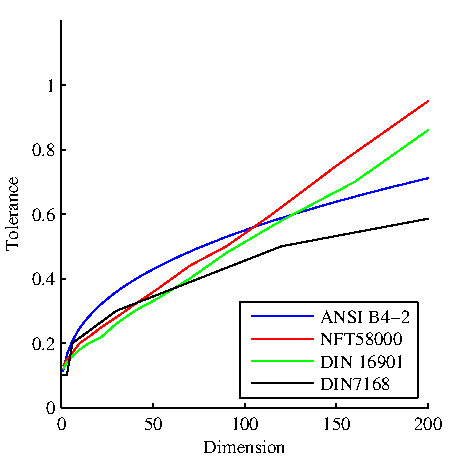
\includegraphics{Tolerance_standards.pdf}
\caption{\label{fig:tolstd}Standards for relation of dimension and tolerance.}
\end{figure}

These standards are all described in technical reports using tables to show the tolerance for a given dimension interval and precision. In a note for \citeauthor{american1978preferred} and later mentioned in \citeauthor{ISO286} a continuous function is described for international tolerance (IT) grades (precision levels) between IT6 and IT16 for dimensions from $2 \ mm$ to $500 \ mm$. This function is for unknown reasons not included in newer versions of \citeauthor{ISO286} yet table values still seem estimated using this function. The relationship is as follows

\begin{align}
	d=& \frac{10^{0.2 (ITG -1)} \cdot i}{2} \\
	i =& 0.45 \sqrt[3]{T} + 10^{-3} \, T 
\end{align}

where $i$ is the standard tolerance factor, $T$ is the target dimension in $[mm]$ and d half specification width in $[\mu m]$. We use said function to normalize the PCSL because the \citeauthor{ISO286}  is widely used in the industry. Further work on improving the normalisation of tolerances or simply choosing the best tolerance specification standard requires more data than we have been able to generate in our test case described in section \ref{sec:result}. The IT grade (ITG) for the measurement set presented in table \ref{tab:sampleset} can be computed

\begin{align*}
&\mathrm{ITG} = 5 \cdot \log_{10} \left\{ \frac{2d \cdot 10^3}{ 0.45  T^{\frac{1}{3}} + T \cdot10^{-3} }\right\} +1 \mathrm{IT grade}\\
&\mathrm{ITG_{specified} } = 13.4 \mathrm{IT grade}\\
&\mathrm{ITG_{actual}}  = 12.5 \mathrm{IT grade}
\end{align*}

$\mathrm{ITG_{actual}}$ is based on the process capability by replacing $d$ with $PCSL$, the process capability driven symmetric tolerance. $\mathrm{ITG_{specified}}$ is the IT grade specified in the design. A lower actual IT grade than the specified IT grade means that the process is performing within the tolerance limits.

\subsubsection{Analyze normalized data}
A further analysis of the underlying measurement sets is done to present the user with an easier to use data view. Relevant measurement sets are aggregated based on design attributes selected by the user.

To help the user determine which tolerance to use, an accumulated frequency plot of the process capability IT grade distribution is proposed. This gives an overview of the current process capability for the selected design attributes. The plot shows the probability to produce the selected part at the specified $C_{pk}$ and tolerance, see figure \ref{fig:acumfreq}.

\begin{figure}
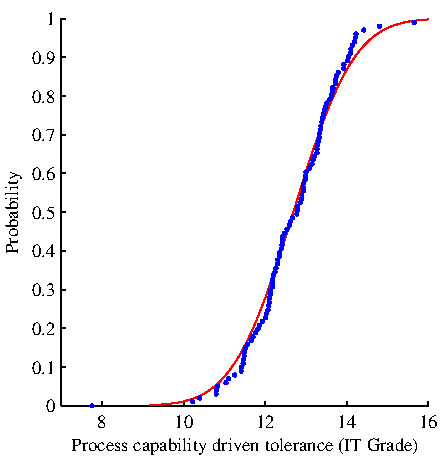
\includegraphics{ITG_total.pdf}
\caption{\label{fig:acumfreq} Accumulated frequency of IT grade distribution with Wilson score confidence intervals.  }
\end{figure}

To even out random effects in the measurements sets, a normal distribution fitted and Wilson score confidence intervals are added based on the number of measurements sets, to show statistical certainty. The IT grades distribution is assumed to be normally distributed due the central limit theorem, which from our sample data seems to be correct, see figure \ref{fig:normplot}. Based on the experience gained from our test data the 90\% cumulative probability should be the standard tolerance grade used for designing new parts. 

The reason for choosing 90\% cumulative frequency and not 100\% is due to a large degree of exceptions in the upper 10\% of the measurements sets. These exceptions include dimensions of: long and slender objects, unnecessary tight tolerances in non-critical areas and dimensions where specifications have become desynchronised from manufacturing targets.

As a designer it is often temping to use an IT grade at a lower cumulative probability, however statistically this will result in errors. Instead the designer should try to specify the given design characteristics more precisely for the given task, hoping these will result in a tighter permissible tolerances.

If a tolerance associated with a low probability of occurrence is chosen generally this will impact the price of production since it either: Increases risks of rework to hit the target $C_pk$ or requires more precise machines than what is used for the measured components.

\begin{figure}
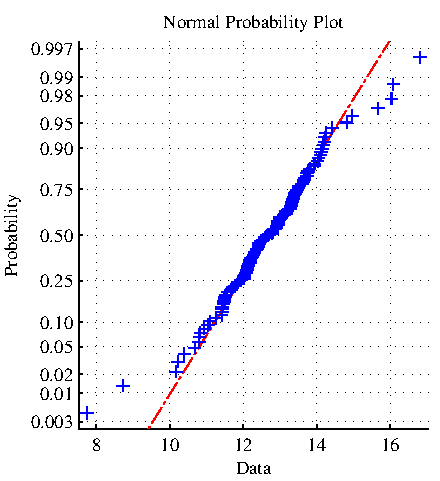
\includegraphics{Normal_plot.pdf}
\caption{\label{fig:normplot} Normality investigation of IT grade of measurement data.}
\end{figure}

\subsection{Statistical Validity}
The user needs to trust the information provided by the PCDB. The uncertainty of the resulting distribution of IT grades is influenced by several factors.

\begin{itemize}
\item More samples in each measurement set will increase certainty. 
\item More measurements sets increase certainty. 
\item Lower standard deviation of the IT grade distribution will increase certainty.
\item Higher mean deviations from target Ca will slightly increase certainty especially at low sample sizes. 
\end{itemize}
Sample size and number of measurement sets are the only two possible actionable variables. 

\subsubsection{Monte Carlo simulation}
To model the uncertainty and accuracy of the IT grade distribution, we have chosen to use Monte Carlo simulation, since it would be very difficult to accurately model analytically. We assume that the IT grade from each measurement set is a continuous random variable with mean $\mu_{\mathrm{ITG}}$ and standard deviation $\sigma_{\mathrm{ITG}}$ giving $\mathrm{ITG} \sim \mathcal{N} (\mu_{\mathrm{ITG}}, \sigma_{\mathrm{ITG}}^2)$.

The randomly generated ITG is converted into a normal distribution of individual measurements X using a fixed target dimension of $T = 100 \mathrm{\ [mm]}$ and closeness to target $C_a = 0.6$. 
The standard deviation $\sigma_{X}$ and mean shift $| \mu - m|$ can be calculated yielding the distribution parameters $\mathrm{X} \sim \mathcal{N} (| \mu - m|, {\mu_{\mathrm{X}}}^2)$. 

Each measurement is generated from the measurement set distribution. When all measurements have been generated the process is reversed and the distribution parameters of the ITG are estimated. The simulation is run $N$ times. 

The Monte Carlo simulation predicts that the standard deviation of the IT grade distribution is overestimated especially at lower sample sizes due the increased uncertainty of these. Even at sample sizes of 10 it is still overestimated by 10\%. This effect can also be seen on figure \ref{fig:confidenceIntervals}, the results of a simulation run with the following parameters: $\mathrm{ITG} ~ N (10, 1)$, sample sizes = 10, number of sample sets = 20, $N$ = 10 000.  

Using the Monte Carlo simulation found that the standard deviation of the IT grade distribution is overestimated especially at lower sample sizes dues the increased uncertainty of these. 
Even at sample sizes of 10 it's still overestimated by 10 \%. 
This effect can be seen on figure \ref{fig:confidenceIntervals}. The mean value is within 1 \% of the original value and is independent of sample size and number of measurements.  

The Monte Carlo simulations were also used to estimate the confidence intervals at different cumulative probabilities using the percentile method. The percentile method interval is the interval between the $ 100 \cdot \alpha$ and $100 \cdot (1 − \alpha)$ percentiles of the Monte Carlo distribution. 
To verify the simulation we compared the confidence intervals to a simple approximation of the interval based on the Wilson score interval, as seen in figure \ref{fig:confidenceIntervals}. The Monte Carlo interval width is very close to the Wilson score at midsection of the probability curve. The confidence intervals for the Wilson score deviates at the top and bottom section, which is a property of the Wilson approximation.

\begin{figure}
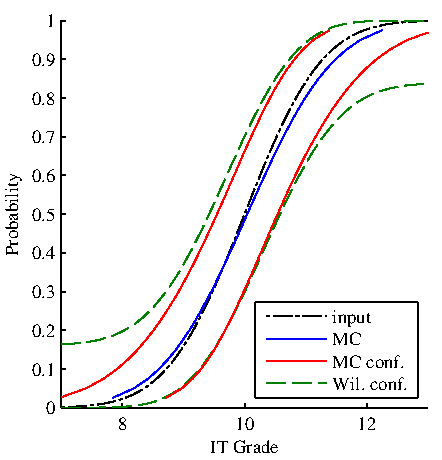
\includegraphics{confidenceIntervals.pdf}
\caption{\label{fig:confidenceIntervals} Monte Carlo cumulated frequency plot.}
\end{figure}

The Monte Carlo simulation were also used to estimated the confidence intervals at different cumulative probabilities using the percentile method.
The percentile method interval is the interval between the $100 \cdot \alpha$ and $100 \cdot (1-\alpha)$ percentiles of the Monte Carlo distribution. 

To verify the simulation we compared the confidence intervals to a simple approximation of the interval based on the Wilson score interval for the same input at the Monte Carlo, as can be seen in Figure \ref{fig:confidenceIntervals}. The Monte Carlo interval width is very close to the wilson score at midsection of probability curve. 
The confidence intervals for the Wilson score deviates at the top and bottom section which is a property of the wilson approximation.

The effects of sample size and number of measurement sets is displayed in Figure \ref{CLW90_lines.pdf}, which shows the symmetric confidence interval at a cumulative probability of $90\%$ as a function of sample size and number of measurement sets. Increasing the sample size only have an effect up to about 12 samples, additional sample measurements do not increase accuracy. The amount of measurement sets is the main factor for reducing the confidence intervals. If the purpose is to differentiate between design attributes then the number of measurement sets is going to limit how small the differences between design attributes can be resolved with statistical certainty.

\begin{figure}
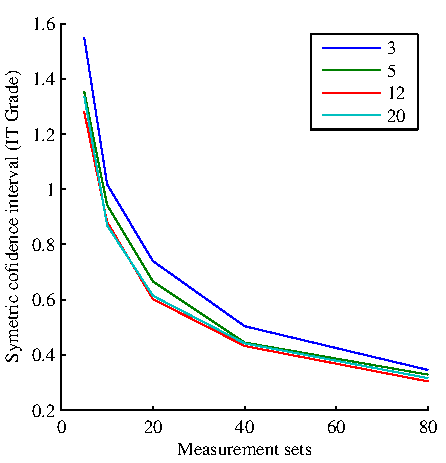
\includegraphics{CLW90_lines.pdf}
\caption{\label{fig:cl_line} Monte Carlo simulation of a normal distribution of IT-grades. The plot shows the symetric cofidence interval size at 90\% probability as a function of both sample size and number of measurement sets. 
The number of sample sets has much bigger influence than sample size for sizes above 12 samples. }
\end{figure}

\section{Result from test case}
\label{sec:result}

To test the concept an experimental database were made. Vaavud, a small company making anemometers, provided technical drawings, samples and inspection reports. Danish Technological Institute provided additional measurements made using their Zeiss CT scanning equipment. The tested parts were all injection moulded. Three parts were made of POM (PTFE filled) in a multi cavity mould. The last part was made using a blend of PC and ABS.

\subsection{Results}

The $90\%$ cumulative frequency of all measurements corresponds to a $14.2 \pm 0.4 \mathrm{IT grade}$. In order to find design attributes with lower minimum permissible tolerances we investigated mould properties, materials, geometries etc. 

\begin{itemize}
\item Linear dimensions within a single mould half did not show significant better performance than dimensions across mould split lines. 
\item Linear dimension performed to the same IT grade level as radii and diameters.
\item Internal and external diameters and radii showed no significant difference.
\item Small ($0-5 \ mm$), medium ($5-10 \ mm$) and large dimensions ($10+ \ mm$) performed to the same required tolerance, though the largest dimension were only 80 mm.
\end{itemize}

We found a very small (or non-existent) correlation between the specified tolerance and the actual process capability driven tolerance, as seen in figure \ref{fig:ITG_ITGSpec}. Which means it makes little or no difference if you apply specified tolerance to each measurement on a part drawing. This clearly shows the need for process capability driven tolerances as a part of robust design. Given the available data, a new part produced using the same production method and materials should be given a tolerance no tighter than 14.2 IT grade. 

Having a database with easy sortable production data can also be used for finding general trends, which can benefit the designer and will be valuable to the production directly. E.g. we found that holes were larger than specified compared to shafts using the mean shift normalised with the specification limit, see figure \ref{\label{fig:Cb_holeshaft}}. This is likely a deliberate choice by the mould maker, since subsequent tool wear will reduce this systematic deviation from target. Further more corrections will be cheap, since it does not require the making of a new mould part. 

\begin{figure}
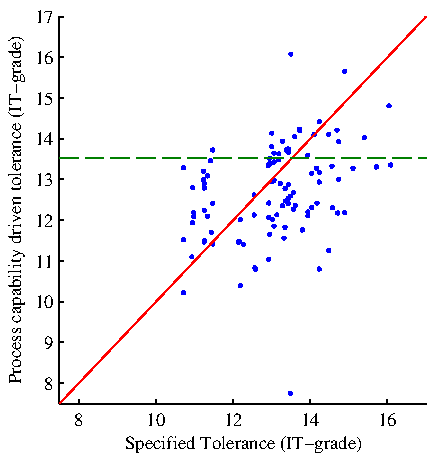
\includegraphics{ITG_ITGSpec.pdf}
\caption{\label{fig:ITG_ITGSpec} Correlation between specified tolerances and actual tolerances. 
Data points above the full line is measurements that exceed the specified tolerance. 
The dotted line represents 90\% cumulative frequency.}
\end{figure}

\begin{figure}
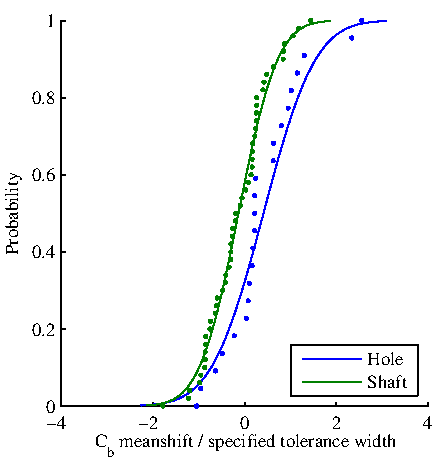
\includegraphics{Cb_holeshaft.pdf}
\caption{\label{fig:Cb_holeshaft} The mean shift normalised with the specification limit of inner measurements such as holes and cavities compared against outside measurements such as shafts, rods and cubes. }
\end{figure}



\section{Conclusion}
In this paper, a review of literature has shown problems in using process capability databases for design purposes. An efficient indexing scheme and easy to use user interface are two key factors to a functional process capability database.

We have proposed a statistical approach for making process capability independent of dimension and an approach for calculating a process capability driven tolerance. The statistical uncertainty has been estimated using Monte Carlo simulation and compared to known statistical approximations.

In the test case we compared different design attributes and in general no significant differences were found. For new designs using the same process and material the minimum tolerance should be 14.2 IT grade. Failure of designing for process capabilities of the production can lead to additional cost for rework or larger failure rate of products.

When designing a new component the generalised process capability database will provide easy access to information of the process capability of the given material and process.

\section*{References}
\bibliography{../PCDBmasterBibliography/PCDB_Master_bib.bib}

\end{document}